\documentclass[twocolumn]{scrartcl}
\usepackage[cm]{fullpage}
\usepackage{hyperref}
\usepackage{graphicx}
\usepackage[backend=biber]{biblatex}
\addbibresource{report.bib}

\title{Classification of wine}
% Do NOT write your names here!
\author{Anonymous Authors}
\begin{document}
\maketitle

\section{Introduction}

The following report outlines our attempts to use common classification
algorithms to predict the wine quality depending on the given features.
We use a data set from the UCI Machine Learning Repository
\footnote{\url{http://archive.ics.uci.edu/ml/datasets/Wine+Quality}} \parencite{data}.

\subsection{Data Description}

The data set contains of 4898 data points, each of them described by 11 features
and an integer quality label ranging from 3 to 9.
Note that the distribution of the quality is unbalanced:
More than 90\% of the data points are assigned to a quality between 5 and 7 (Figure \ref{fig:unbal}).

\begin{figure}[h]
    \centering
    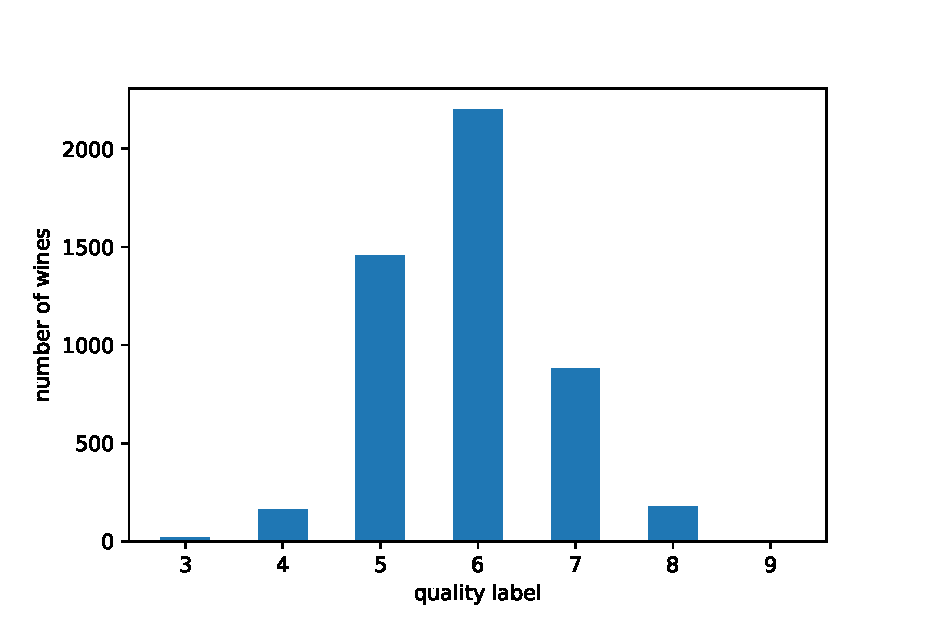
\includegraphics[width=\linewidth]{images/unbalanced.eps}
    \caption{distribution of quality}
    \label{fig:unbal}
\end{figure}

\subsection{Data preprocessing}

To simplify our problem we assigned new class labels 0, 1 and 2. We assign class 0 (bad) to wines ranging in qualities 3-5,
class 1 (medium) to wines labeled with quality 6 and class 2 (good) to wines with quality greater than 6.
We further decided to use classification instead of regression.
Though, it should be noted that we also examine algorithms (e.g. ridge classifier) that use regression to classify the data points
and using regression should therefore yield similar results in our case.
This doesn't come as a surprise, considering that the classes can obviously be linearly ordered.

%not yet decided which to use
\section{Ridge Classification}
\subsection{Description}
\subsection{Cross-Validation}
\subsection{Results}

\section{Multi Layer Perceptron}
\subsection{Description}
\subsection{Cross-Validation}
\subsection{Results}

\section{Random Forest Classification}
\subsection{Description}
\subsection{Cross-Validation}
\subsection{Results}

\section{Gaussian Process Classification}
\subsection{Description}
\subsection{Cross-Validation}
\subsection{Results}

\section{Comparison}
\section{Conclusion}

\printbibliography

\end{document}
